
\section{Introduction}\label{sec:introduction}
The customer's demands on the Naiad AUV included that there should be sensors for the pressure, temperature and salinity of the surrounding water. These readings are needed for two reasons: 

\begin{itemize}
\item The speed of sound in water is needed to get accurate positional readings from sensors such as sonar and hydrophones. Since these only measure the time it takes for sound to travel a certain distance, multiplication by the speed of sound gives the distance travelled by the sound.

\item The salinity of the water will affect the density of the water. Given an estimation of the density of the water a pressure reading will give an estimation of the depth of the AUV. This reading will not be affected by drift (unlike for example inertial sensors).

\end{itemize}

A Generic CAN controller was used to handle the sensors. The \emph{Generic CAN controller} is a small (approx. 76 by 40 millimetres) electronic board that has an AT90CAN128 microcontroller~\cite{web:at90can}, an MCP2551 CAN transceiver~\cite{web:mcp2551} and all the peripheral circuitry needed for these as well as its own power supply. The Generic CAN controller is used throughout the project for several tasks. It can be connected to the CAN bus and has two UART buses as well as an SPI bus. \newline
An electronic board known as the \emph{Sensor Controller Board} was built to provide an electrical interface between the sensors and the Generic CAN controller. The Sensor Controller Board is "stacked" on top of the Generic CAN controller. This structure can be seen in Figure~\ref{fig:sensor_overview}.  \newline
The AT90CAN128 microcontroller on the Generic CAN controller runs a program known as the \newline
\emph{AT90CAN\_Sensor\_Controller} that reads the sensor values and outputs their readings on the CAN bus.

Due to the financial situation of the project, the salinity sensor was never purchased and because of this no circuitry or software regarding  the salinity sensor could ever be tested. 

\begin{figure}[h]
    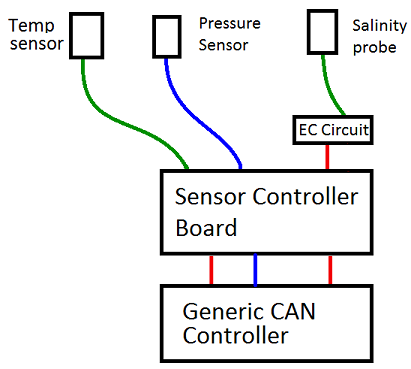
\includegraphics[width=0.5\textwidth]{./figure/sensor_overview.png}
    \caption{The structure of the Sensor Controller. Blue lines indicate 1-Wire interfaces, green lines are analog interfaces and red lines are UART interfaces.}
    \label{fig:sensor_overview}
\end{figure}